\scanpage{63}

Notons d'ailleurs, pour le cas d'un entier $n$ ne satisfaisant \unsure{pas \inserted{nécessairement}|\inserted{nécessairement} pas} les conditions envisagées dans c):

\uline{Corollaire} \inserted{10}. Soit $n$ un entier. On a alors une suite exacte canonique
\margin{\figure{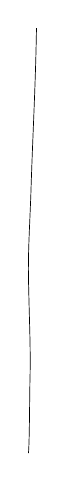
\begin{tikzpicture}[x=.596685cm,y=.596685cm,line width=.25pt]
\draw (0.17,9.05) .. controls (0.15,7.80) and (0.09,6.80) .. (0.05,5.50)
 .. controls (0.02,4.70) and (-0.01,4.30) .. (0.00,3.70)
 .. controls (0.02,2.70) and (0.05,2.20) .. (0.03,1.50)
 .. controls (0.02,0.80) and (0.02,0.30) .. (0.00,0.00);
\end{tikzpicture}}}
\diagram{$(1\deleted{0}\inserted{1})\qquad$\begin{tikzcd}[ampersand replacement=\&,column sep=small]
0\arrow[r]\&{}_n\Gamma\arrow[r]\&H^1(X,\mu_n)\arrow[r,"u_n"]\&H^1(X_{\bar\eta},\mu_n)^I\arrow[r]\&Q_{\deleted{\unsure{n|a}}}(n)\arrow[r]\&0,
\end{tikzcd}}
où $Q_n=\operatorname{Coker}u_n$ s'insère dans une suite exacte canonique
\diagram{$(1\deleted{\unsure{0|1}}\inserted{2})\qquad$\begin{tikzcd}[ampersand replacement=\&,column sep=small]
0\arrow[r]\&\operatorname{Ker}w_n\arrow[r]\&Q_{\deleted{\unsure{n|a}}}(n)\arrow[r]\&\unsure{\theta|\Theta}(n)\arrow[r]\&0,
\end{tikzcd}}
avec
\[
(1\deleted{2}\inserted{3})\qquad\unsure{\theta|\Theta}(n)\hookrightarrow{}_n\operatorname{Ker}(\operatorname{Br}(K)\longrightarrow\operatorname{Br}(X_\eta))\hookrightarrow{}_{(n,d^t)}\operatorname{Br}(K),
\]
\margin{\begingroup
\setbox0=\hbox{$\hookrightarrow$}
\dimen0=\wd0 \advance\dimen0 by 8pt
\dimen2=\ht0 \advance\dimen2 by \dp0 \advance\dimen2 by 8pt
\leavevmode\rlap{\raisebox{\dimexpr-\dp0-4pt\relax}{%
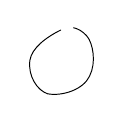
\begin{tikzpicture}[x={\dimexpr\dimen0/217\relax},y={\dimexpr\dimen2/152\relax},line width=.35pt]
\path[use as bounding box] (0,0) rectangle (217,152);
\begin{scope}[shift={(-7,37)}]
\draw (112,110) .. controls (65,94) and (20,70) .. (14,43)
 .. controls (7,8) and (38,-24) .. (70,-31)
 .. controls (118,-37) and (183,-21) .. (202,8)
 .. controls (224,38) and (213,81) .. (193,97)
 .. controls (179,108) and (164,113) .. (151,115);
\end{scope}
\end{tikzpicture}}}%
\kern4pt\box0\kern4pt\endgroup}
de sorte que l'on a $\unsure{\theta|\Theta}(n)=0$ lorsque $n$ ou $d^t$ sont premiers à $p$ ou\deleted{\unsure{r|k|x}} que $k$ est parfait (donc $\operatorname{Br}(K)=0$). En tous cas, si $p^m$ est la plus grande puissance de $p$ divisant $d^t$ (qui est donc indépendant du choix de $n$), on a
\[
(1\deleted{\unsure{3|2}}\inserted{4})\qquad p^m\unsure{\theta|\Theta}(n)=0\qquad\text{pour tout }n.
\]
Pour $n$ variable multiplicativement, les \deleted{\unsure{suites}} diagrammes (1\deleted{0}\inserted{1}), (1\deleted{\unsure{0|1}}\inserted{2}) et (1\deleted{2}\inserted{3}) forment des systèmes projectifs, pour des morphismes de transition évidents, \deleted{et on a, grâce grâce}

Si donc $n$ parcourt lespuissances d'un nombre premier fixé $\ell$, alors il résulte de (1\deleted{\unsure{3|2}}\inserted{4}) que $\varprojlim_{\unsure{\nu|\gamma}}\unsure{\theta|\Theta}(\ell^\nu)=0$, \deleted{de sorte que par passage à la limite à partir de\unsure{s}} donc $\varprojlim_{\unsure{\nu|\gamma}}\operatorname{Ker}w_{\ell^{\unsure{\nu|\gamma}}}\unsure{\simeq|\xrightarrow{\sim}}\varprojlim Q(\ell^\nu)$ \deleted{, et} par (1\deleted{\unsure{1|0}}\inserted{2}), d'où la suite exacte (7) par passage à la limite à partir de (\deleted{\unsure{9|10}}\inserted{11}).\begin{tikzpicture}[overlay,x=.006cm,y=-.006cm]\draw[line width=.45pt] (-49,2) .. controls (-50,31) and (-47,67) .. (-48,112);\draw[line width=.35pt] (-35,2) .. controls (-32,27) and (-35,51) .. (-33,81);\end{tikzpicture}

Nous prouverons également le

\uline{Corollaire} 15. Posons
\[
(16)\qquad d^{\unsure{t|f}}=p^r a,\qquad\text{avec }(a,p)=1.
\]
Alors il existe un \deleted{revêtement} ddagramme
\diagram{$(\inserted{17})\qquad$\begin{tikzcd}[ampersand replacement=\&]
\unsure{\deleted{O}X|X|M}\arrow[d,"f"']\&X'\arrow[l,"h"']\arrow[d,"f'"]\\
S\&S',\arrow[l,"g"']
\end{tikzcd}}
avec $h$ un revêtement étale \begingroup
\setbox0=\hbox{\begingroup\let\sout\relax\deleted{principal de groupe $\unsure{G_a|g|G}$}\endgroup}
\leavevmode\rlap{\begin{tikzpicture}[overlay,baseline=0pt,x={\dimexpr\wd0/574\relax},y={\dimexpr\wd0/574\relax},line width=.35pt]
\draw (3,15) .. controls (12,23) and (22,7) .. (35,8)
 .. controls (100,13) and (135,18) .. (170,11)
 .. controls (240,4) and (315,-1) .. (365,5)
 .. controls (430,14) and (455,1) .. (485,-2)
 .. controls (535,-6) and (562,-6) .. (574,6);
\draw (10,15) .. controls (18,0) and (4,-8) .. (6,-28);
\draw (14,6) .. controls (100,-3) and (164,-9) .. (218,4);
\draw (574,6) .. controls (571,-5) and (565,-13) .. (562,-25);
\end{tikzpicture}}
\box0\endgroup, $S'\longrightarrow S$ un revêtement

\margin{62}
